% Format teze zasnovan je na paketu memoir
% http://tug.ctan.org/macros/latex/contrib/memoir/memman.pdf ili
% http://texdoc.net/texmf-dist/doc/latex/memoir/memman.pdf
% 
% Prilikom zadavanja klase memoir, navedenim opcijama se podešava 
% veličina slova (12pt) i jednostrano štampanje (oneside).
% Ove parametre možete menjati samo ako pravite nezvanične verzije
% mastera za privatnu upotrebu (na primer, u b5 varijanti ima smisla 
% smanjiti 
\documentclass[12pt,oneside]{memoir}

% Paket koji definiše sve specifičnosti mastera Matematičkog fakulteta
\usepackage[latinica]{matfmaster}
%
% Podrazumevano pismo je ćirilica.
%   Ako koristite pdflatex, a ne xetex, sav latinički tekst na srpskom jeziku
%   treba biti okružen sa \lat{...} ili \begin{latinica}...\end{latinica}.
%
% Opicija [latinica]:
%   ako želite da pišete latiniciom, dodajte opciju "latinica" tj.
%   prethodni paket uključite pomoću: \usepackage[latinica]{matfmaster}.
%   Ako koristite pdflatex, a ne xetex, sav ćirilički tekst treba biti
%   okružen sa \cir{...} ili \begin{cirilica}...\end{cirilica}.
%
% Opcija [biblatex]:
%   ako želite da koristite reference na više jezika i umesto paketa
%   bibtex da koristite BibLaTeX/Biber, dodajte opciju "biblatex" tj.
%   prethodni paket uključite pomoću: \usepackage[biblatex]{matfmaster}
%
% Opcija [b5paper]:
%   ako želite da napravite verziju teze u manjem (b5) formatu, navedite
%   opciju "b5paper", tj. prethodni paket uključite pomoću: 
%   \usepackage[b5paper]{matfmaster}. Tada ima smisla razmisliti o promeni
%   veličine slova (izmenom opcije 12pt na 11pt u \documentclass{memoir}).
%
% Naravno, opcije je moguće kombinovati.
% Npr. \usepackage[b5paper,biblatex]{matfmaster}

% Pomoćni paket koji generiše nasumičan tekst u kojem se javljaju sva slova
% azbuke (nema potrebe koristiti ovo u pravim disertacijama)
\usepackage{pangrami}

% Paket koji obezbeđuje ispravni prikaz ćiriličkih italik slova kada
% se koristi pdflatex. Zakomentarisati ako na sistemu koji koristite ovaj
% paket nije dostupan ili ako ne radi ispravno.
\usepackage{cmsrb}

% Ostali paketi koji se koriste u dokumentu
\usepackage{listings} 

\lstdefinelanguage{JavaScript}{
  morekeywords=[1]{break, continue, delete, else, for, function, if, in,
    new, return, this, typeof, var, void, while, with},
  % Literals, primitive types, and reference types.
  morekeywords=[2]{false, null, true, boolean, number, undefined,
    Array, Boolean, Date, Math, Number, String, Object},
  % Built-ins.
  morekeywords=[3]{eval, parseInt, parseFloat, escape, unescape},
  sensitive,
  morecomment=[s]{/*}{*/},
  morecomment=[l]//,
  morecomment=[s]{/**}{*/}, % JavaDoc style comments
  morestring=[b]',
  morestring=[b]"
}[keywords, comments, strings]

\lstalias[]{ES6}[ECMAScript2015]{JavaScript}

\lstdefinelanguage[ECMAScript2015]{JavaScript}[]{JavaScript}{
  morekeywords=[1]{await, async, case, catch, class, const, default, do,
    enum, export, extends, finally, from, implements, import, instanceof,
    let, static, super, switch, throw, try},
  morestring=[b]` % Interpolation strings.
}

% Requires package: color.
\definecolor{mediumgray}{rgb}{0.3, 0.4, 0.4}
\definecolor{mediumblue}{rgb}{0.0, 0.0, 0.8}
\definecolor{forestgreen}{rgb}{0.13, 0.55, 0.13}
\definecolor{darkviolet}{rgb}{0.58, 0.0, 0.83}
\definecolor{royalblue}{rgb}{0.25, 0.41, 0.88}
\definecolor{crimson}{rgb}{0.86, 0.8, 0.24}

\lstdefinestyle{JSES6Base}{
  backgroundcolor=\color{white},
  basicstyle=\ttfamily,
  breakatwhitespace=false,
  breaklines=false,
  captionpos=b,
  columns=fullflexible,
  commentstyle=\color{mediumgray}\upshape,
  emph={},
  emphstyle=\color{crimson},
  extendedchars=true,  % requires inputenc
  fontadjust=true,
  frame=single,
  identifierstyle=\color{black},
  keepspaces=true,
  keywordstyle=\color{mediumblue},
  keywordstyle={[2]\color{darkviolet}},
  keywordstyle={[3]\color{royalblue}},
  numbers=left,
  numbersep=5pt,
  numberstyle=\tiny\color{black},
  rulecolor=\color{black},
  showlines=true,
  showspaces=false,
  showstringspaces=false,
  showtabs=false,
  stringstyle=\color{forestgreen},
  tabsize=2,
  title=\lstname,
  upquote=true  % requires textcomp
}

\lstdefinestyle{JavaScript}{
  language=JavaScript,
  style=JSES6Base
}
\lstdefinestyle{ES6}{
  language=ES6,
  style=JSES6Base
}

% Datoteka sa literaturom u BibTex tj. BibLaTeX/Biber formatu
\bib{matfmaster}

% Ime kandidata na srpskom jeziku (u odabranom pismu)
\autor{Aleksa Kojadinović}
% Naslov teze na srpskom jeziku (u odabranom pismu)
\naslov{Arhitektura i dizajn veb platforme za upravljanje korisničkim žalbama i zahtevima}
% Godina u kojoj je teza predana komisiji
\godina{2023}
% Ime i afilijacija mentora (u odabranom pismu)
\mentor{Vladimir Filipović}
% Ime i afilijacija prvog člana komisije (u odabranom pismu)
\komisijaA{Saša Malkov}
% Ime i afilijacija drugog člana komisije (u odabranom pismu)
\komisijaB{Aleksandar Kartelj}
% Ime i afilijacija trećeg člana komisije (opciono)
% \komisijaC{}
% Ime i afilijacija četvrtog člana komisije (opciono)
% \komisijaD{}
% Datum odbrane (obrisati ili iskomentarisati narednu liniju ako datum odbrane nije poznat)
\datumodbrane{xx. januar xxxx.}

\setcounter{tocdepth}{3}


% Apstrakt na srpskom jeziku (u odabranom pismu)
\apstr{%
\pangrami
}

% Ključne reči na srpskom jeziku (u odabranom pismu)
\kljucnereci{veb, DDD, servis, API, analitika}

\begin{document}
% ==============================================================================
% Uvodni deo teze
\frontmatter
% ==============================================================================
% Naslovna strana
\naslovna
% Strana sa podacima o mentoru i članovima komisije
\komisija
% Strana sa posvetom (u odabranom pismu)
% Strana sa podacima o disertaciji na srpskom jeziku
\apstrakt
% Sadržaj teze
\tableofcontents*

% ==============================================================================
% Glavni deo teze
\mainmatter
% ==============================================================================

% ------------------------------------------------------------------------------
\chapter{Uvod}
% ------------------------------------------------------------------------------
% \pangrami

\section{Veb platforme}
\section{Sistem STS}

Svaki biznis koji neku vrstu usluge pruža korisnicima neizostavno mora imati korisničku podršku u nekom obiku. Pre razvoja veb tehnologija telefonski sistemi bili su jedini način direktne podrške koju korisnik može da dobije. Razvoj i pristupčanost veba doveli su do evolucije vrlo sofisticiranih onlajn proizvoda koji rešavaju problem korisničke podrške, kako putem pisanih rasprava u vidu tiketa, tako i dalje putem tradicionalnih telefonskih linija uz određenu integraciju\footnote{\href{http://zendesk.com}{Zendesk}, \href{https://www.8x8.com/}{8x8}, \href{https://www.atlassian.com/software/jira/service-management}{Jira Service Management}}.

Sistem STS\footnote{Skraćeno od eng. Simple Ticket Service, jednostavan servis za tikete}, razvijan za potrebe ovog rada, obuhvata osvnovnu funkcionalnost za pružanje podrške u vidu tiketa. Tiket predstavlja jednu tekstualnu korisničku žalbu ili zahtev, na kojoj se može pokrenuti diskusija, a sve sa ciljem asinhronog\footnote{pod asinhronošću podrazumevano suprotnost u odnosu na telefonski sistem gde korisnik i agent podrške vode komunikaciju u realnom vremenu.} razrešenja korisničkog problema. Glavni akteri sistema su:

\begin{itemize}
    \item \textbf{Mušterije} - koje mogu postavljati tikete u cilju dobijanja podrške
    \item \textbf{Agenti} - koji su zaduženi da odgovaraju na tikete, upravljaju njihovim statusima, i rešavaju probleme
    \item \textbf{Administratori} - zaduženi za podešavanje sistema, dodeljivanje uloga korisnicima, zabranu pristupa korisnicima, ili uopšteno bavljenje kompleksnim problemima 
\end{itemize}

\subsection{Osnovne funkcionalnosti, prikaz tiketa, statusi}

Osnovni pojam sistema, kao što je pomnuto, jeste tiket. Na slici možemo videti primer zaglavlja jednog tiketa. Sastoji se primarno iz naslova i opisa, dok se takođe može videti i ime mušterije, i trenutno zaduženog agenta.

\begin{figure}[h]
  \centering
  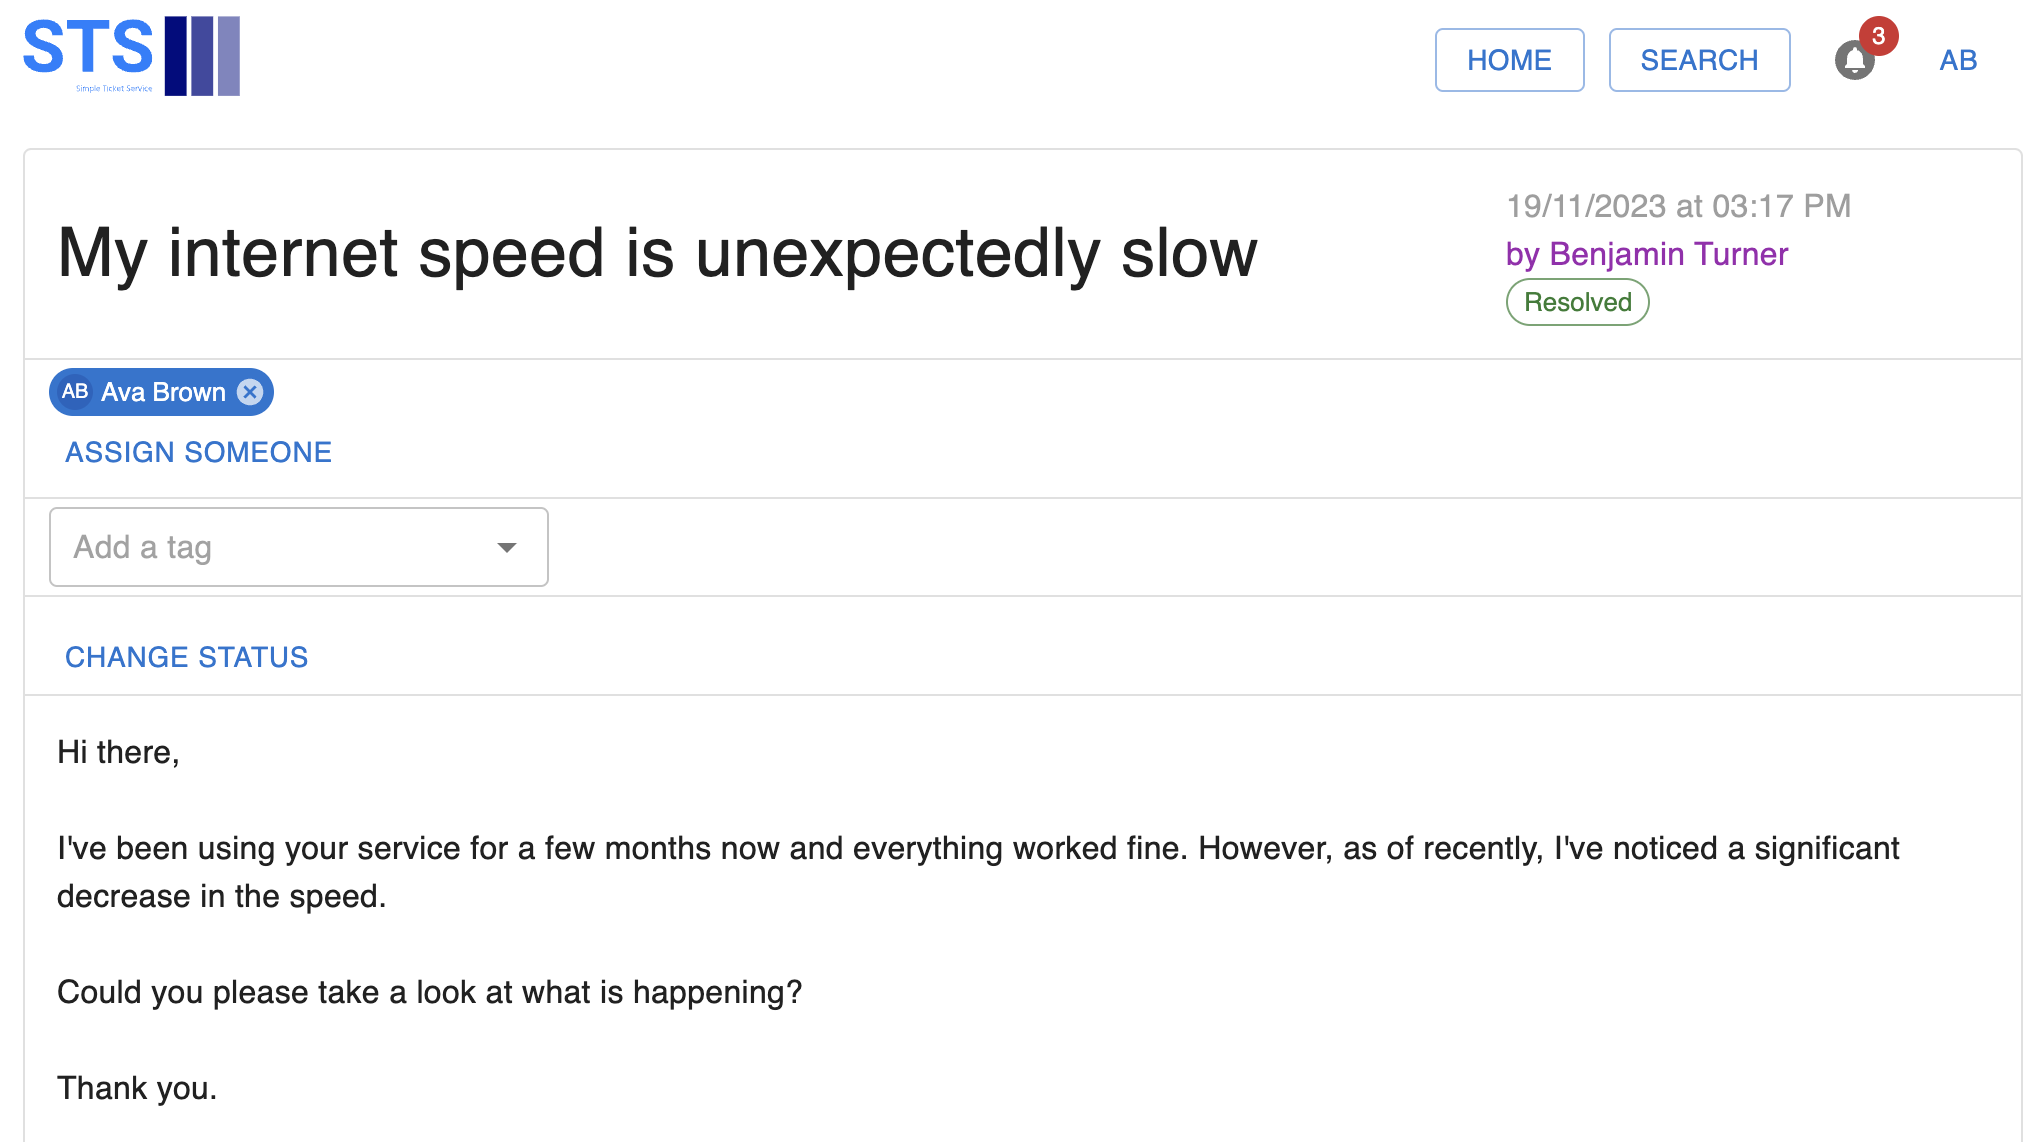
\includegraphics[width=1\textwidth]{docs/images/ch_1/ticket-title.png} 
  \caption{Primer tiketa.}
\end{figure}

Tiket može prolaziti kroz više statusa, i promene tih statusa vidljive su kako agentima tako i korisnicima

\begin{figure}[h]
  \centering
  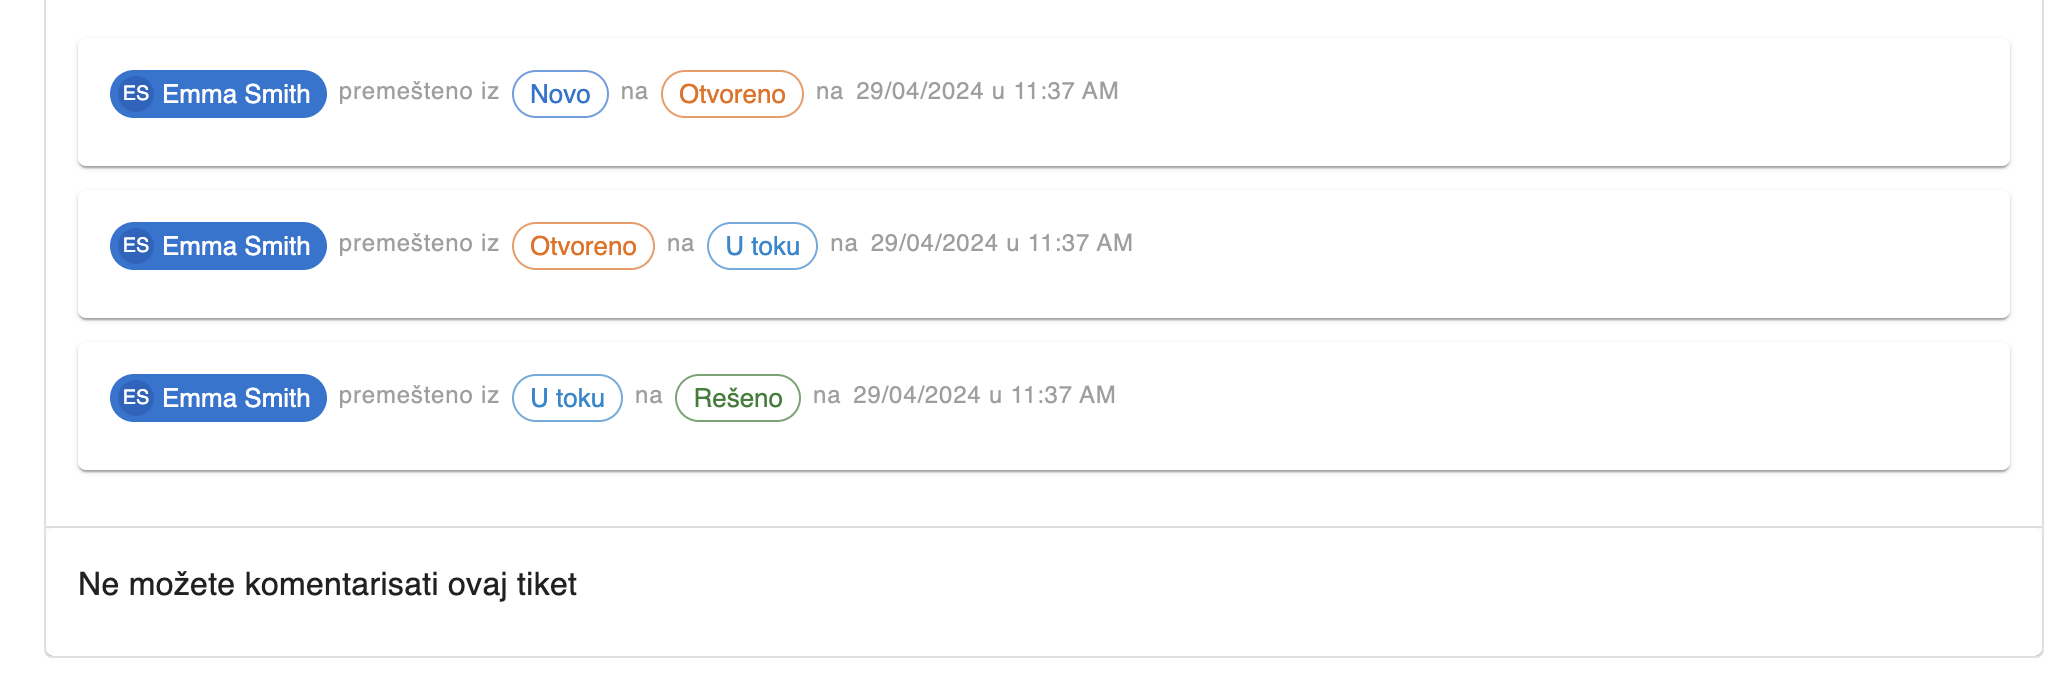
\includegraphics[width=1\textwidth]{docs/images/ch_1/ticket-statuses.png} 
  \caption{Promene statusa.}
\end{figure}

\subsection{Sistem oznaka, konfigurabilnost}

Često postoji potreba klasifikacije tiketa po raznim kriterijumima - departman unutar firme koji se bavi tiketom, hitnost, prioritetnost, i slično. Kako bi se postigla maksimalna fleksibilnost uveden je sistem oznaka (eng. tags). Oznaka se može nakačiti na dati tiket i može dati brzu informaciju o nekim njegovim aspektima. Ovaj sistem u potpunosti je konfigurabilan od strane korisnika (u ovom slučaju administratora), tako da nije potrebna intervencija programera prilikom dodavanja novih ili promene postojećih oznaka.

Na sledećoj slici vidimo kako izgleda tiket označen oznakama histnosti i odeljenja.

\begin{figure}[h]
  \centering
  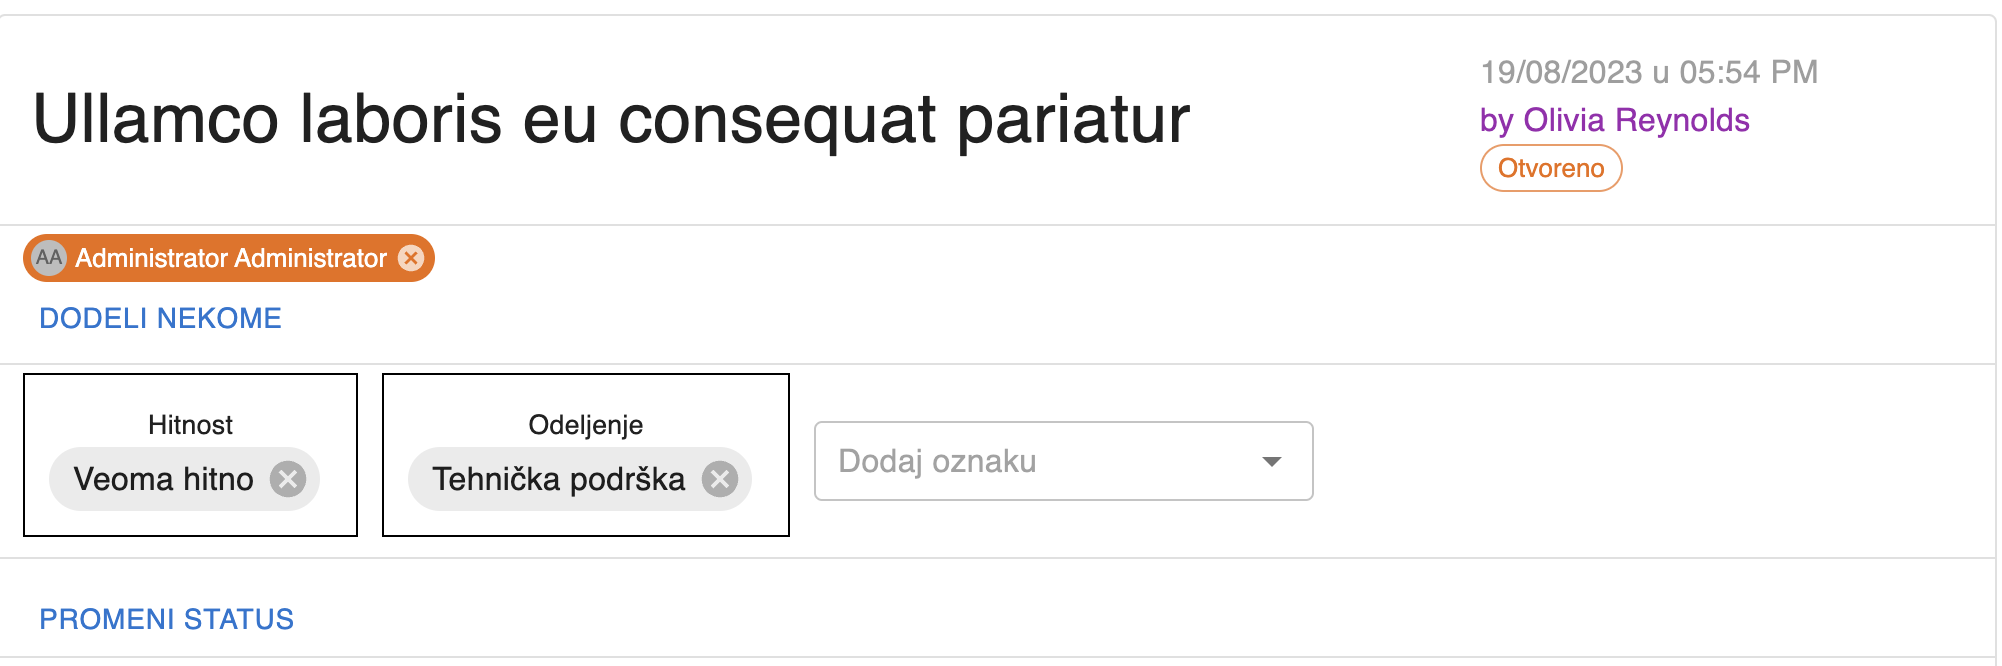
\includegraphics[width=1\textwidth]{docs/images/ch_1/tagged-ticket.png} 
  \caption{Tiket sa oznakama hitnosti i odeljenje.}
\end{figure}

Sledeće dve slike prikazuju kontrolnu tablu na kojoj administatori mogu upravljati oznakama. Primećujemo dodatnu fleksibilnost u sistemu kojom se može konfigurisati koji tip korisnika ima pravo da vidi, dodaje i uklanja koju oznaku. Takođe primećujemo da sistem podržava višejezičnost, tako što se imena i opisi mogu podešavati i na srpskom i na engleskom jeziku. O jezicima i sistemu internacionalizacije biće više reči u sekciji \ref{sec:intl}.

\begin{figure}[h]
  \centering
  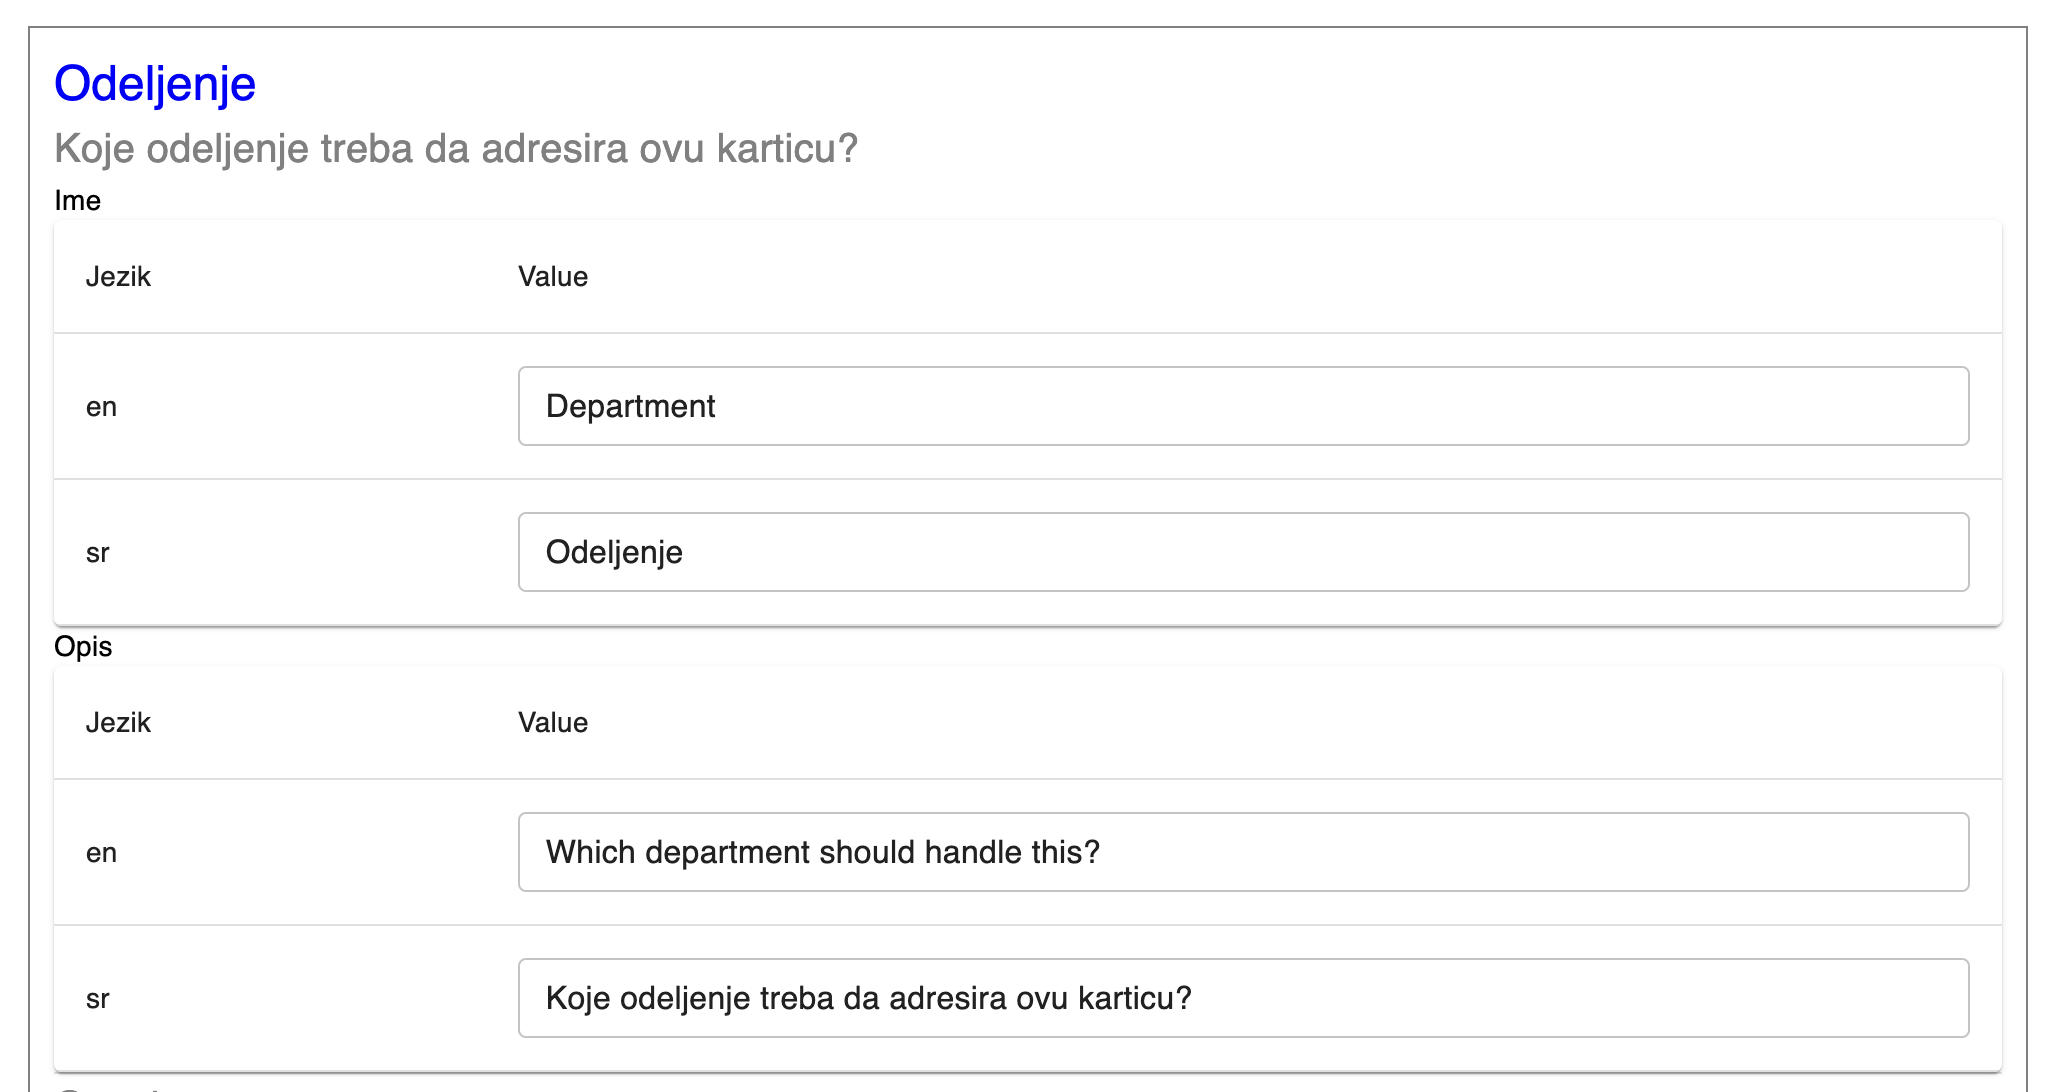
\includegraphics[width=1\textwidth]{docs/images/ch_1/tag-mgmt-head.png} 
  \caption{Kreiranje oznake, višejezička imena.}
\end{figure}

\begin{figure}[h]
  \centering
  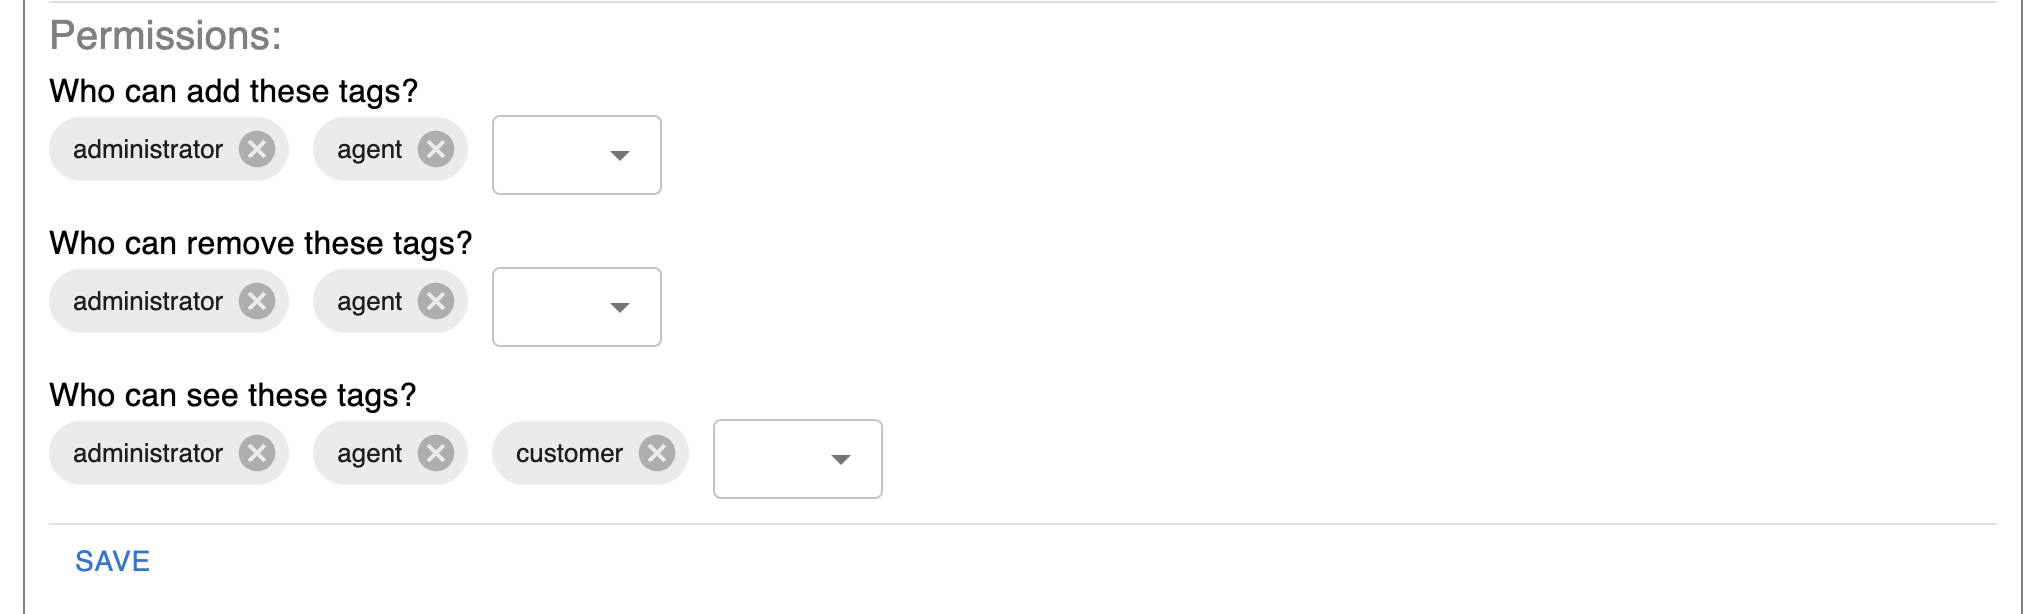
\includegraphics[width=1\textwidth]{docs/images/ch_1/tag-mgmt-permissions.png} 
  \caption{Kreiranje oznake, permisije.}
\end{figure}

\newpage
\subsection{Upravljanje korisnicima}

Administratori poseduju mogućnost upravljanja korisnicima sajta, putem kontrolne table na adresi \textit{manage/users} koja prikazuje listu svih korisnika i akcije koje mogu biti primenjene nad njima. Od akcija podržana je promena tipa korisnika (pod određenim uslovima), i promena statusa korisnika.

\begin{figure}[h]
  \centering
  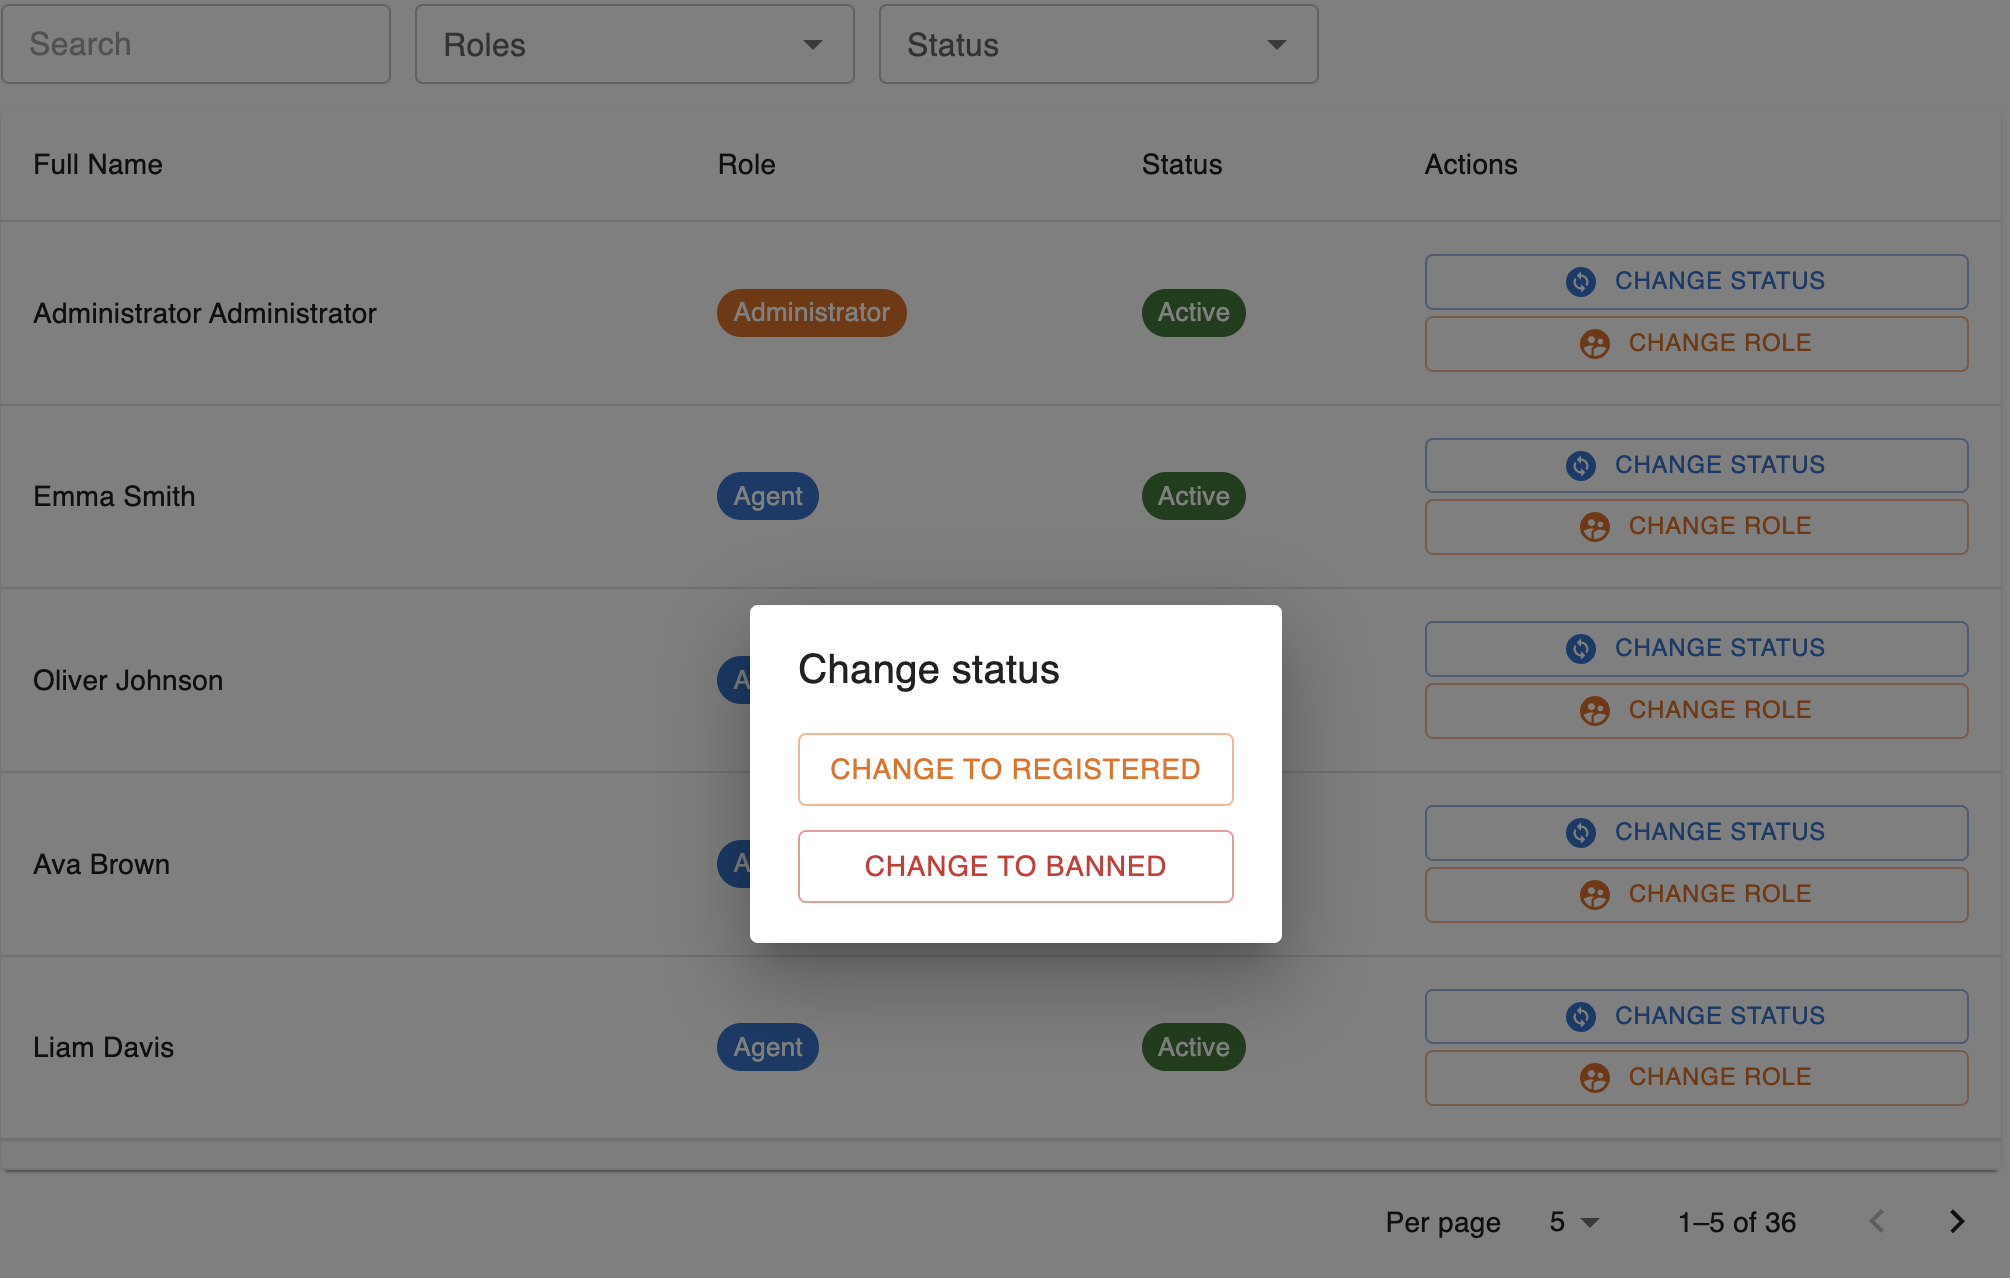
\includegraphics[width=1\textwidth]{docs/images/ch_1/manage-users-preview.png} 
  \caption{Upravljanje korisnicima.}
\end{figure}



\newpage
\section{Višeservisno okruženje}

% ------------------------------------------------------------------------------
\chapter{Bekend}
% ------------------------------------------------------------------------------
Kod velikog broja softverskih sistema, serverski deo aplikacije (bekend) može se uopšteno shvatiti kao aplikacija koja apstrahuje pristup podacima na udaljenom serveru. Podaci se skoro uvek čuvaju u nekoj vrsti baze podataka, dok se pristup i manipulacija podacima dodatno apstrahuje aplikativnim\footnote{Opštosti radi, izbegnuti su pojmovi \textbf{veb server} i \textbf{http server}. Veb server predstavlja server za dostavljanje statičkog sadržaja na vebu, i često kada govorimo o bekend aplikacijama ne mislimo na ovaj tip servera (nginx, apache2). HTTP server takođe ne bi bio ispravan pojam usled postojanja drugih protokola komunikacije na vebu} serverom.

Navedeni gradivni delovi - baza podataka i aplikativni server - tehnički su dovoljni za implementaciju bekend dela aplikacije. Mnogi kursevi razvoja veb aplikacija, pogotovu oni zasnovani na MEAN i MERN\footnote{Mongo, Angular ili React, Express, Node.js, dve popularne kombinacije veb tehnologija} okruženjima, upravo ovakve primere i prikazuju. Tu neretko srećemo arhitekturu od samo dva sloja - sloj aplikativnog programskog interfejsa (eng. Application Programming Interface - API) i sloja pristupa bazi podatka. Međutim, za izgradnju složene aplikacije koja uzima u obzir čistoću k\^{o}da, razdvajanje odgovornosti, održivost, i iskustvo programera (eng. Developer Experience - DX) potrebno je dodatno raslojiti aplikaciju i pratiti neke ustanovljene principe.


\section{DDD}
Jedan od najpopularnijih pristupa za dizajn i modelovanje softvera jeste dizajn zasnovan na domenu (eng. Domain Driven Design - DDD). Ukratko, DDD zagovara detaljno upoznavanje svih učesnika razvoja softvera sa domenom koji dati softverski sistem predstavlja. Programeri u saradnji sa domenskim stručnjacima razvijaju zajednički, sveprisutan jezik (eng. ubiquitous language) kako bi se prevazišla barijera različitog rečnika svih strana. \cite{dddq}

\subsection{Korišćenje domenskog jezika u programskom k\^{o}du}
\label{sec:dddukodu}
Nakon uspostavljanja, sveprisutan jezik postaje sastavni deo komunikacije programera i domenskih stručnjaka (i svih ostalih učesnika razvoja), ali isto tako i programskog k\^{o}da. Naime, programski k\^{o}d koji nastaje kao produkt modelovanja principa DDD-a postaje jasniji i dostiže viši stepen samodokumentovanosti. U takvom k\^{o}du sama imena klasa, metoda i promenljivih mogu biti dovoljna da programeru daju jasnu sliku šta koja celina k\^{o}da radi. Upravo zbog ovoga, primena DDD-a nije ograničena samo na velike kompanije ili velike timove, i ne služi samo kao sredstvo prevazilaženja "jezičkih" barijera, već doprinosi čistoći k\^{o}da i arhitekture i u manjim timovima, čak i jednočlanim. U sledeća dva primera prikazan je deo metode koja vrši ažuriranje komentara na tiketu. Primer 2.1 prikazuje ovu metodu pisanu ne uzimajuću domenski jezik u obzir.


\begin{figure}[h]
\begin{lstlisting}[language=JavaScript, style=ES6, caption={K\^{o}d koji nije na domenskom jeziku}]
function updateComment(...){
  const ticket = //...
  
  if (!ticket) {
    throw new NotFoundException('Ticket not found.');
  }

  if (ticket.status === TicketStatus.CLOSED ||
      ticket.status === TicketStatus.RESOLVED) {
    throw new BadRequestException('Ticket closed.')
  }

  if (user.role === Role.CUSTOMER &&
      ticket.createdBy.id !== user.id) {
    throw new ForbiddenException('Not your ticket');
  }
  
  const comment = //...
  
  if (!comment) {
    throw new NotFoundException('Comment not found.')
  }
  
  if (comment.user.id !== user.id) {
    throw new ForbiddenException('Not your comment.');
  }
}
\end{lstlisting}
\end{figure}
\newpage
Odlikuje se ručnim proverama identifikacionih polja i direktnim podizanjem HTTP grešaka unutar servisa. Iako može biti razumljiv u toku pisanja, ovakva vrsta k\^{o}da u kompleksnom sistemu postaje neodrživa.

\begin{figure}[h]
\begin{lstlisting}[language=JavaScript, style=ES6, caption={K\^{o}d koji je na domenskom jeziku}]
function updateComment(...) {
  const ticket = // ...

  if (!ticket) {
    throw new TicketNotFoundError(ticketId);
  }

  if (ticket.isFinalStatus()) {
    throw new CannotChangeTicketInFinalStatusError(ticket.status);
  }

  if (user.isCustomer() && !ticket.isOwner(user)) {
    throw new CannotCommentOnOthersTicketsError();
  }

  const comment = // ...

  if (!comment) {
    throw new CommentNotFoundError();
  }

  if (!comment.isOwner(user)) {
    throw new CannotUpdateOthersCommentsError();
  }
}
\end{lstlisting}
\end{figure}

\newpage
U ovom primeru primećujemo prisustvo domena u svim aspektima. Metode kao što su $isFinalStatus$ i $isOwner$ i semantičke klase grešaka kao \textit{CannotChangeTicketInFinalStatus} doprinose da određeni delovi k\^{o}da dostižu nivoe čitljivosti bliske prirodnom jeziku.

\subsection{Slojevita arhitektura}
Prilikom izrade softvera, usled rokova i nedostatka resursa, neretko dolazi do isprepletanosti poslovne logike, logike korisničkog interfejsa, logike pristupa bazi podataka i drugih komponenti sistema \cite{dddfull}. Ovakve odluke u razvoju, iako rezultuju kratkoročnim rešenjem, dugoročno dovode do borbe sa onim što kolokvijalno nazivamo \textit{tehnički dug}\footnote{eng. technical debt}. Postojanje tehničkog duga se takođe javlja iz drugih odluka tokom razvoja i u praksi je pokazano da opšte rešenje ovog problema ne postoji; svaki tim se pre ili kasnije sretne sa tehničkim dugom koji otežava i usporava rad. Ipak, ta neminovnost ne treba da obeshrabri rano uvođenje dobrih praksi kao što je raslojavanje arhitekture. 

DDD razaznaje četiri sloja, s tim što u ovom pogavlju razmatramo prva tri, dok je sloj korisničkog interfejsa predmet narednog poglavlja. Detaljna diskusija o slojevima, uz relevantnu implementaciju, prikazana je u sekcijama 2.2, 2.3 i 2.4.

\begin{figure}[h]
  \centering
  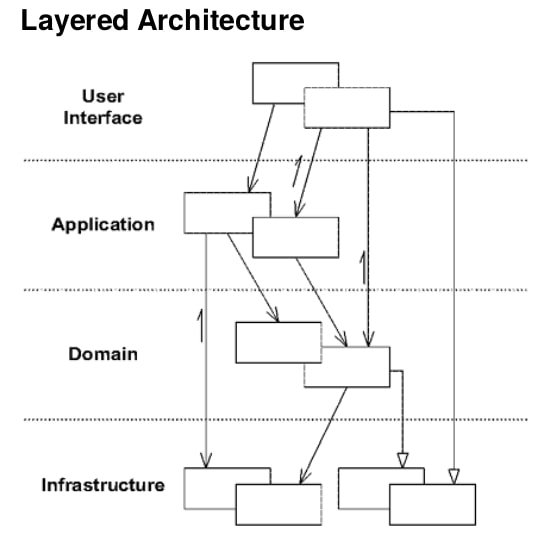
\includegraphics[width=0.5\textwidth]{docs/images/ch_2/DDD-Layered-Architecture-2.png} 
  \caption{Slojevi sistema \cite{dddfull}}
  \label{fig:sample}
\end{figure}

\section{Okruženje NestJS}

NestJS \cite{nestjsdocs} je Node.js okruženje za razvoj serverskih aplikacija. Izgrađen je nad bibliotekom \textit{express} \cite{expressjsdocs} koja je i danas popularan izbor za izradu manjih serverskih aplikacija, kao i za edukativne svrhe.  U srž ovog okruženja ugrađeni su koncepti modula, servisa i umetanja zavistnosti (eng. Dependency Injection - DI), što ga čini idealnim za konstrukciju aplikacije zasnovane na DDD principima.

Osnovni gradivni elementi NestJS aplikacije su \textit{moduli}. Svaki modul obuhvata jednu smislenu celinu aplikacije koja može sadržati \textit{kontrolere} i \textit{provajdere}. U slučaju DDD-a, modul odgovara jednom izolovanom kontekstu\footnote{eng. Bounded Context \cite{dddfull}}. Module definišemo na deklarativni način, pri čemu u okviru modula možemo uvoziti i druge module kako bismo postigli saradnje različitih delova sistema.

\begin{figure}[h]
\begin{lstlisting}[language=JavaScript, style=ES6, caption={fajl tickets.module.ts}]
@Module({
  // Sekcija koja uvozi ostale module
  imports: [
    MongooseModule.forFeature(...),
    UsersModule,
    TicketTagSystemModule,
    NotificationsModule,
  ],
  // Sekcija koja deklarise kontrolere
  controllers: [TicketsController],
  // Sekcija koja deklarise servise i repozitorijume
  providers: [
    TicketService,
    TicketCommentService,
    TicketRedactionService,
    TicketTagUpdateService,
    TicketAssigneesService,
    TicketsRepository,
  ],
})
export class TicketsModule {}
\end{lstlisting}
\end{figure}

Kao što vidimo sa primera, NestJs se jako oslanja na metaprogramiranje i mogućnosti jezika \textit{typescript} u vidu dekoratora. Prilikom pokretanja NestJS aplikacije vrši se korak poznat kao \textbf{bootstrap}, odnosno priprema aplikacije za rad. U tom koraku se razrešavaju sve međuzavisnosti modula i servisa i instanciraju sve klase kojima se upravlja putem umetanja zavisnosti.

Što se tiče strukture direktorijuma i fajlova u okviru projekta, korišćen je hibrid između mnogo sistema viđenih u praktičnom radu, a takav da najbolje odgovara i zahtevima okruženja, i sistema koji modelujemo. Primer strukture prikazan je u nastavku.

\begin{figure}[h]
\begin{lstlisting}[language=JavaScript, style=ES6, caption={fajl tickets.module.ts}]
|-- api/
|   |-- dto/
|   |-- profiles/
|-- domain
|   |-- entities/
|   |-- errors/
|   |-- services/
|   |-- value-objects/
|-- infrastructure
    |-- interceptors/
    |-- schema/
\end{lstlisting}
\end{figure}

\section{Sloj infrastrukture}

Sloj infrastrukture ima više uloga u DDD sistemu, ali zajednička osobina je odsustvo iniciranja akcija u sloju domena \cite{dddfull}. Veliki deo ovog sloja često zauzima implementacija trajnosti podataka (eng. data persistence), i to neretko šablonom repozitorijuma (eng. Repository pattern). Uloga ovog šablona jeste odvajanje logike za čuvanje podataka van domenskog modela \cite{msrepository}. Često se ostvaruje uz pomoć jedne ili više klasa sa nekim uobičajenim metodama za dohvatanje ili ažuriranje entiteta.


\subsection{Repozitorijumi}
Apstrakcija koju pruža sloj repozitorijuma ogleda se upravo u načinu na koji on obrađuje podatke pre vraćanja u više slojeve, tačnije služi se \textbf{šablonom preslikavanja podataka} (eng. Data mapper pattern). Uloga mapiranja podataka uglavnom je u praksi delegirana konkretnoj biblioteci ili okruženju, koja upravlja pristupom bazi putem softverskog segmenta iz klase Objektno-relacionih ili Objektno-dokumentnih preslikavača (eng. Object Relational Mapper - ORM, Object Document Mapper - ODM). Iako ti sistemi često u potpunosti zadovoljavaju potrebe mapiranja podataka, u ovom radu je mapiranje urađeno manuelno, tako da se objekti dobijeni ODM slojem, odnosno bibliotekom \textit{mongoose} \cite{mongoosedocs}, preslikavaju u entitete koristeći biblioteku \textit{@automapper/js} \cite{automapperjsdocs}.

\begin{figure}[h]
  \centering
  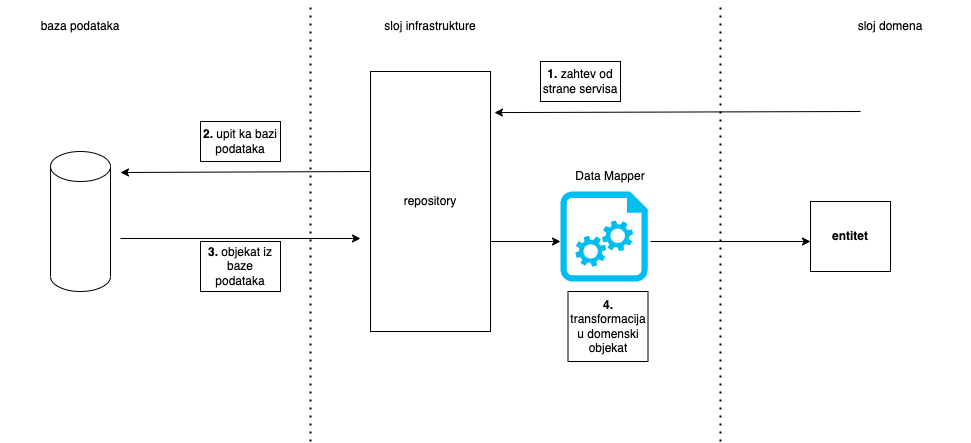
\includegraphics[width=1\textwidth]{docs/images/ch_2/repository.png} 
  \caption{Dijagram dohvatanja entiteta preko repozitorijuma}
  \label{fig:sample}
\end{figure}

Prirodno se nameće pitanje dohvatanja povezanih entiteta, ili konkretnije rad sa agregatima. U ovom radu implementiran je sistem \textbf{pohlepnog učitavanja} (eng. eager loading), kojim se svi povezani entiteti zahtevanog entiteta dohvataju odmah prilikom zahteva ka glavnom entitetu. U nekim sistemima ovakav izbor ne bi bio idealan, međutim takva odluka je doneta u ovoj situaciji usled činjenice da je dizajn baze podataka relativno jednostavan, i lakoća implementacije i korišćenja nadmašuje cene u performansama, koje su minimalne. Kombinacijom metode $populate$ 
 i biblioteke \textit{mongoose} i rekurzivne prirode biblioteke \textit{automapper/js} ovo se lako postiže.

Na sledećem isečku vidimo zaglavlje klase \textit{TicketsRepository}. Kao i sve ostale repozitorijumske klase, oslanjaju se na model klase dobijene od strane biblioteke \textit{mongoose}, i deklarišu niz koji predstavlja sve putanje koje treba popuniti zarad implementacije pohlepnog učitavanja.

\begin{figure}[h]
\begin{lstlisting}[language=JavaScript, style=ES6, caption={Fajl \textit{tickets.repository.ts}, konstrukcija i niz POPULATE}]
export class TicketsRepository {
  constructor(
    @InjectModel() private ticketModel: Model<TicketDb>,
    @InjectMapper() private readonly mapper: Mapper,
  ) {}

  public static POPULATE = [
    {
      path: 'history.initiator',
      model: 'UserDb',
    },
    {
      path: 'history.payload.assignees',
      model: 'UserDb',
    },
    { path: 'createdBy', model: 'UserDb' },
    {
      path: 'tags',
      model: 'TicketTagDb',
      populate: { path: 'group', model: 'TicketTagGroupDb' },
    },
    { path: 'assignees', model: 'UserDb' },
  ];
\end{lstlisting}
\end{figure}

\newpage
Sledeći isečak prikazuje primer dohvatanja jednog tiketa putem identifikatora, pri čemu se, naravno, prilikom vraćanja rezultata vrši mapiranje u odgovarajući entitet.

\begin{figure}[h]
\begin{lstlisting}[language=JavaScript, style=ES6, caption={Fajl \textit{tickets.repository.ts}, dohvatanje entiteta}]
async findById(id: string): Promise<Ticket | null> {
    const result = await this.ticketModel
      .findById(id)
      .populate(TicketsRepository.POPULATE);
    
    if (!result) {
      return null;
    }
    
    return this.mapper.map(result, TicketDb, Ticket);
}
\end{lstlisting}
\end{figure}

\newpage
\subsection{Sheme, mutacije podataka, šablon Event Sourcing}
Osim repozitorijuma, sloj infrastrukture prirodno sadrži i definicije shema biblioteke \textit{mongoose}. Iz ugla programera, ovi objekti su najbliža pristupna tačka bazi podataka i podržavaju operacije upita i mutacija nad realnim podacima u bazi. Takav jedan upit viđen je na isečku 2.4 u prethodnoj sekciji.

Na ovom mestu bavimo se mutacijama podataka, i to baš tiketa. Osim prikaza rada sa mutiranjem podataka kroz biblioteku \textit{mongoose}, ovaj primer služi da ilustruje dualnu prirodu tiketa kao entiteta i njegovu potpunu različitost u strukturi između sloja infrastruktura i sloja domena. Naime, kao što će biti prikazano u sledećem poglavlju, tiket u sloju domena je jednostavna klasa koja sadrži sve podatke o datom tiketu. Ipak, u sloju infrastrukture, radi veće fleksibilnosti i mogućnosti praćenja istorije, upotrebljena je varijanta šablona \textit{Event Sourcing}. Osnovno načelo ovog šablona je da umesto čuvanja eksplicitnog stanja objekta čuvamo istoriju njegovih promena.

Na sledećem isečku vidimo deo klase koja predstavlja shemu za rad sa tiketima.

\begin{figure}[h]
\begin{lstlisting}[language=JavaScript, style=ES6, caption={Fajl \textit{ticket.schema.ts}}]
@Schema({ collection: "tickets" })
export class TicketDb extends Document {
  _id: string;

  @Prop({ type: Date })
  createdAt: Date;

  @Prop({ type: String })
  title: string;

  @Prop({ type: String })
  body: string;

  @Prop({ type: String })
  status: TicketStatus;

 // ...

  @Prop({ type: [{ type: mongoose.Schema.Types.Mixed }] })
  history: TicketHistoryItem[];
}
\end{lstlisting}
\end{figure}


\newpage
Niz \textit{history} predstavlja promene primenjene na datom tiketu, na osnovu kojih se može izvesti trenutno stanje tiketa. Ipak, prirodno se postavlja pitanje zašto se, osim istorije promena, čuvaju i eksplicitna polja kao što su \textit{status}, \textit{title}, \textit{body} i drugi, budući da se ti podaci mogu izvući putem istorije. Razlog leži u performansama pretrage. Ukoliko bismo čuvali samo listu promena, a ne sliku trenutnog stanja (eng. snapshot), svaka pretraga bi bila linearne vremenske složenosti u odnosu na dužinu istorije, što bi rezultovalo lošim performansama.

Sa ovakvom postavkom, mutacije nad tiketom postižu se diferencijacijom prosleđenog entiteta i entiteta iz baze podataka.

\begin{figure}[h]
\begin{lstlisting}[language=JavaScript, style=ES6, caption={Fajl \textit{ticket.repository.ts}}]
  async update(newTicket: Ticket, user: User) {
    const document = await this.ticketModel
      .findById(newTicket.id)
      .populate(TicketsRepository.POPULATE); 

    const timestamp = new Date();

    // Trenutno stanje tiketa
    const ticket = this.mapper.map(document, TicketDb, Ticket);

    // Primer diferencijacije nad poljem title
    if (newTicket.title !== ticket.title) {
      const item = new TicketHistoryItem();
      item.initiator = user.id as unknown as UserDb;
      item.timestamp = timestamp;
      item.type = TicketHistoryEntryType.TITLE_CHANGED;

      // Dodajemo novu stavku u istoriju
      item.payload = 
         new TicketHistoryEntryTitleChanged(newTicket.title);
         
      document.history.push(item);
      // Menjamo snapshot stanje
      document.title = newTicket.title;
    }
\end{lstlisting}
\end{figure}

Za kraj, na primeru komentara nad tiketom, prikazujemo uprošćenu verziju mapiranja iz oblika u sloju infrastrukture u domenski entitet, dok se puna verzija nalazi u izvornom k\^{o}du u fajlu \textit{ticket.entity-profile.ts}.

\begin{figure}[h]
\begin{lstlisting}[language=JavaScript, style=ES6, caption={Mapiranje komentara tiketa}]
  forMember((destination) => destination.comments,
    mapFrom((source) => {
      const commentItems = source.history.filter(
        (item) => item.type === COMMENT_ADDED,
      );

      return commentItems
        .map((item) => {
          // pretrzujemo sve komentare u istoriji
          const payload = item.payload as CommentAdded;
          // proveravamo da li su kasnije bili obrisani
          const deletes = source.history.filter(
            (deleteItem) => deleteItem.type === COMMENT_DELETED 
            && (deleteItem.payload as CommentDeleted)
                .commentId === payload.commentId,
            );
          
          const wasDeleted = deletes.length > 0;

          if (wasDeleted) {
            return null;
          }

          // ... mapiranje samog komentara u domenski oblik...

          return comment;

\end{lstlisting}
\end{figure}




\newpage
\section{Sloj domena}

Takođe poznat kao srce poslovnog softvera, sloj domena sadrži glavnu poslovnu logiku i operacije koje direktno oslikavaju dešavanja u svetu koji softver modeluje. Iz ugla implementacije, svoje mogućnosti pružaju putem apstrakcije koju često nazivamo servisima, što koristimo i kao sufiks u nazivima njihovih klasa, iako se mogu koristiti i druge konvencije\footnote{Nekad se umesto sufiksa \textit{Service} koriste reči koje direktno oslikavaju namenu datog servisa. Na primer umesto \textit{GetUserService} koristi se naziv \textit{UserProvider} i sl.}.

\subsection{Tok podataka kroz domenski sloj}

Usled činjenice da obuhvata sve poslovne operacije, nije lako definisati opštu namenu domenskog sloja. Na slici 2.3 prikazan je uopšten primer toka podataka kroz ovaj sloj i njemu susedne slojeve.

\begin{figure}[h]
  \centering
  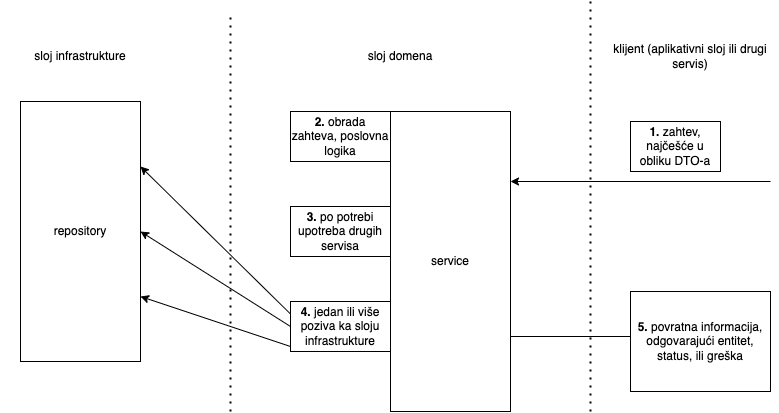
\includegraphics[width=1\textwidth]{docs/images/ch_2/domain.png} 
  \caption{Uopšteni tok obrade podataka kroz domenski sloj}
  \label{fig:sample}
\end{figure}

Ipak, operacije unutar servisa (koraci 2-4) konkretizovaćemo za potrebe sistema kojim se bavimo, jer se mogu svesti na sledeći šablon, gde redosled ne mora nužno biti ispraćen u k\^{o}du usled prirode jezika\footnote{Zbog asinhrone prirode okruženja Node.js, radi postizanja maksimalnih performansi, neke operacije pokrećemo paralelno, a zatim čekamo koristeći funkciju $Promise.all$, što može naizgled delovati kao mešanje koraka.}:

\begin{enumerate}
  \item Dohvatanje odgovarajućeg entiteta
  \item Provera domenskih prava pristupa i domenskih grešaka
  \item Obrada entiteta
  \item Komunikacija sa drugim servisima
  \item Osiguravanje trajnosti podataka
  \item Priprema i vraćanje odgovarajućeg odgovora
\end{enumerate}

Na sledećem primeru operacije dodeljivanja tiketa agentima prikazujemo prethodne korake, redom.

\newpage
\textbf{Dohvatanje entiteta}

\begin{figure}[h]
\begin{lstlisting}[language=JavaScript, style=ES6, caption={dohvatanje tiketa}]
async addAssignees(ticketId: string, user: User, dto: AssignDTO) {
  const ticket = await this.ticketsRepository.findById(ticketId);
  if (!ticket) {
    throw new TicketNotFoundError(ticket.id);
  }
\end{lstlisting}
\end{figure}

\textbf{Provera domenskih prava pristupa i domenskih grešaka}
\begin{figure}[h]
\begin{lstlisting}[language=JavaScript, style=ES6, caption={domenska prava pristupa i greške}]
  // Domensko pravo pristupa - korisnicima nije dozvoljeno
  // dodeljivanje tiketa
  if (user.isCustomer()) {
    throw new NotAllowedToAssignError();
  }
  const assignees: User[] = await Promise.all(
    dto.assignees.map((id) => this.usersService.findOne(id)),
  );

  for (const assigneeUser of assignees) {
    // Greske domenskog karatkera
    if (!assigneeUser) {
      throw new AssigneeNotFoundError();
    }
    if (assigneeUser.isCustomer()) {
      throw new CannotAssignCustomerError(assigneeUser.id);
    }
    if (ticket.isAssigned(assigneeUser)) {
      throw new DuplicateAssigneeError(assigneeUser.id);
    }
}
\end{lstlisting}
\end{figure}

\newpage
\textbf{Obrada entiteta}

U ovom slučaju obrada je jednolinijska, zbog pogodne definicije klase Ticket.
\begin{figure}[h]
\begin{lstlisting}[language=JavaScript, style=ES6, caption={obrada entiteta}]
ticket.assign(assignees);
\end{lstlisting}
\end{figure}

\textbf{Komunikacija sa drugim servisima}

Konstruišemo niz obaveštenja koja je potrebno poslati, slanje delegiramo odgovarajućem servisu.
\begin{figure}[h]
\begin{lstlisting}[language=JavaScript, style=ES6, caption={drugi servisi}]
const usersToNotify = assignees.filter(
  (assignee) => assignee.id !== user.id,
);
const notifications = usersToNotify.map((userToNotify) =>
  NotificationFactory.create((builder) =>
    builder
      .forUser(userToNotify)
      .hasPayload('assigned', (assignBuilder) =>
        assignBuilder.atTicket(ticket).byUser(user),
      ),
  ),
);
const promise = this.notificationsService.emitNotifications(
  ...notifications,
);
\end{lstlisting}
\end{figure}

\textbf{Osiguravanje trajnosti podataka}

Čuvamo načinjene promene u bazi podataka.
\begin{figure}[h]
\begin{lstlisting}[language=JavaScript, style=ES6, caption={trajnost}]
// ...
this.ticketsRepository.update(ticket, user);
\end{lstlisting}
\end{figure}

\newpage
\textbf{Priprema i vraćanje odgovarajućeg odgovora}

Gde pritom koristimo servis \textit{TicketRedactionService} kako bismo otklonili podatke koje dati tip korisnika ne bi trebalo da vidi.
\begin{figure}[h]
\begin{lstlisting}[language=JavaScript, style=ES6, caption={odgovor}]
this.ticketRedactionService.prepareResponse(updatedTicket, user);
return updatedTicket;
\end{lstlisting}
\end{figure}

\newpage
\subsection{Obrada grešaka}

U prethodnom primeru toka podataka primećujemo intenzivan rad sa greškama. Ovom delu posvećena je posebna pažnja jer je obrada grešaka jedno od centralnih pitanja dizajna kompleksnog softverskog sistema i bitno je od početka dizajnirati ga korektno kako bi kasniji rad bio znatno olakšan.

Naime, programer koji se bavi implementacijom odgovarajuće domenske funkcionalnosti pre ili kasnije susrešće se sa potrebom da obrađuje greške. Čak i najjednostavniji zahtev, kao što je, recimo, dohvatanje jednog tiketa, zahteva rad sa greškama na svakom od nivoa slojevite arhitekture. Manuelno orkestriranje grešaka pri svakoj implementaciji neke funkcionalnosti dovelo bi do usporenog rada i nekonzistentnog sistema bez jasnih standarda. 

Stoga pravimo jasnu podelu između grešaka domenskog nivoa i grešaka aplikativnog nivoa (HTTP grešaka), i u domenskom sloju držimo se isključivo grešaka domenskog nivoa. Sve domenske greške nasleđuju sledeću baznu klasu.

\begin{figure}[h]
\begin{lstlisting}[language=JavaScript, style=ES6, caption={BaseError.ts}]
export class BaseError {
  constructor(public message: string = 'An error occurred') {}

  public getName() {
    return this.constructor.name;
  }

  public getPayload(): any {
    return {
      message: this.message,
      errorType: this.getName(),
    };
  }
}
\end{lstlisting}
\end{figure}

Na ovaj način imamo uniforman interfejs kako svaka greška treba da izgleda, sa dovoljno fleksibilnosti da pokrije sve domenske situacije. U k\^{o}du možemo primetiti sve od jednostavnih grešaka koje predstavljaju nepostojanje - primer \textit{TicketNotFound}, do grešaka koje ukazuju na kompleksnu sitaciju - primer \textit{CannotChangeCommentsOfAClosedTicket}. Na ovakav sistem mogu se uložiti nekoliko kritika, koje ćemo razjasniti.

\textbf{Repetitivnost.}  
Sve greške koje se odnose na nepostajanje entiteta imaju identičan oblik, pa se može uložiti primedba na ponavljanje k\^{o}da, i sugerisati kreiranje dodatnih apstrakcija. U ovom radu izbegli smo takav pristup iz dva razloga
\begin{itemize}
    \item \textbf{Bespotrebne apstrakcije}. Iako je tehnički moguće apstrahovati greške nepostajanja entiteta u neki tip višeg nivoa - recimo \textit{EntityNotFoundError}, ovo uvodi previše jezičke kompleksnosti u domenski sloj, i na duge staze ne doprinosi ni čitljivosti ni razumevanju.
    \item \textbf{Fleksibilnost}. Ukoliko svaki entitet ima priliku da definiše svoje greške bez ograničenja međuapstrakcija, postiže se maksimalna fleksibilnost u okviru datog entiteta. Može se argumentovati da ovakav pristup olakšava potencijalni prelaz na mikroservisnu arhitekturu, po potrebi.
\end{itemize}
\textbf{Preterana ekspresivnost.} Na ovom mestu konkretno govorimo o dužini naziva nekih klasa, koje se mogu smatrati nečitljivim. Ipak, ako se podsetimo dela \ref{sec:dddukodu}, jasno nam je da dobitak na razumljivosti domena kroz k\^{o}d nadmašuje strah od dugačkih imena klasa.

Ostaje pitanje transformacije ovakvih grešaka u HTTP oblik. Jedno izrazito elegantno rešenje, koje nam pružaju mogućnosti okruženja NestJs, biće prikazano u sledećem pogavlju.

\subsection{Integracije sa eksternim servisima}

\section{Sloj aplikacije}

Sve do sad razmatrane slojeve i delove sistema možemo smatrati internim u smislu mogućnosti spoljnjeg pristupa - sloj domena bavi se poslovnom logikom, uz podršku sloja infrastrukture. Kako bi domenski sistem mogao da se koristi od strane grafičkih veb aplikacija, mobilnih aplikacija ili uopšteno bilo kojih drugih softverskih sistema, potebno je da svoju funkcionalnost eksponira spoljašnjem svetu. 

\subsection{REST API, svojstva}

Ovo se postiže slojem aplikacije, tankim slojem bez poslovnog znanja čija glavna uloga jeste primanje zahteva i njihova delegacija na domenski sloj \cite{dddfull}. U ovom radu, za potrebe implementacije aplikativnog sloja, bavimo se najpoznatijim arhitekturalnim stilom poznatim kao REST (\textit{\textbf{RE}presentational \textbf{S}tate \textbf{T}ransfer}). Kompletna specifikacija ovog protokola je ogromna, i pokriva sve aspekte korišćenja HTTP-a kao transportnog sloja veb aplikacija, tako da pominjemo samo neke od najvažnijih:

\begin{itemize}
    \item \textbf{Odsustvo stanja.} Jedan moderan princip softverskog inženjerstva (u vreme pisanja ovog rada) jeste da komponente ili moduli sistema treba da imaju što manje stanja, a po mogućstvu da ga u potpunosti eleminišu\footnote{Ovaj princip postaje posebno primetan rastom popularnosti funkcionalnih programskih jezika.}. Način na koji ovo shvatamo u REST sistemima je sledeći - za dva API zahteva pod identičnim uslovima dobija se identičan odgovor. Dakle, ne postoji nikakav eksterni faktor samog aplikativnog sloja koji može uticati na odgovor koji korisnik (klijent) dobije, i smatra se da je klijent dužan da pruži kompletan kontekst potreban za obradu zahteva \cite{restapi}.

    \item \textbf{Identifikacija resursa i HTTP metode.} Neretko u praksi srećemo takozvane API slojeve sa previše ekspresivnim delovima URI-a\footnote{eng. Uniform Resource Identifier - URI}-a. REST definiše nedvosmislen način za identifikaciju resursa i njihovu hijerarhiju, kao i pravilnu upotrebu HTTP metoda (glagola). Na taj način, API pristupna tačka\footnote{eng. API endpoint} koja pruža mogućnost dohvatanja korisnika po identifikatoru po pravilu treba da bude dostupna putem GET metode, i to na URI-u nalik na \textit{api/users/123}\cite{restapi}. Primer nepravilnog URI-a bilo bi direktno navođenje akcije dohvatanja - \textit{api/get-user-by-id/213}. Na sličan način jasno je propisano koje metode se koriste za promenu, upis i brisanje entiteta.

    \item \textbf{Korišćenje HTTP greški.} Kao što je pomenuto u prethodnoj sekciji, obrada grešaka predstavlja vitalan aspekt razvoja softvera, i značaj deo njene implementacije leži u aplikativnom sloju. REST definiše skup pravila za korektno ukazivanje korisniku na greške koje su se dogodile.  
\end{itemize}

\subsection{Kontroleri, validacija, mapiranje}

Većina okruženja za programiranje veb aplikacija, uključujući i NestJS, pruža ugrađen konstrukt za obradu HTTP zahteva koju nazivamo \textbf{kontroler}. Kontroleri su ništa drugo nego klase nad kojim definišemo metode koje obrađuju HTTP zahteve ka određenom URI-u, dok je proces mapiranja URI-a na metodu maksimalno prepušten okruženju, a programeru eksponiran nekim vidom metaprogramiranja (najšće dekoratorima). Naredni primer ilustruje kontroler koji se vezuje za URI prefiks \textit{users}, koji sadrži metodu koja označava reagovanje na dinamički zadat identifikator. Ovako postavljen kontroler obrađuje zahteve oblika \textit{GET /api/users/123}.

\begin{figure}[h]
\begin{lstlisting}[language=JavaScript, style=ES6, caption={primer kontrolera}]
@Controller('users')
export class UsersController {
  @Get(':id')
  findOne(id: number): UserDTO {
    // ...
  }
}
\end{lstlisting}
\end{figure}

Uloga kontrolera je višestruka, i sastoji se od sledećih koraka:
\begin{enumerate}
    \item \textbf{Provera prava pristupa}. Gde pritom ova provera treba da poznaje što manje poslovne logike. Na primer, neke pristupne tačke dostupne su samo ulogovanim korisnicima, neke samo administratorima, i sl.
    \item \textbf{Validacija ulaznih podataka}. Ponovo mislimo na čisto tehničku validaciju, a ne na poslovnu validaciju. Tu spada provera da li su određeni brojčani podaci zaista brojevi, da li su određeni tekstualni podaci dovoljne dužine i slično.
    \item \textbf{Delegacija posla odgovarajućem sevisu}. Nakon uspešne provere prava pristupa i validacije podataka, kontroler će prepustiti zadatak servisu koji je za to namenjem, i po potrebi primiti povratnu informaciju.
    \item \textbf{Obrada servisnih grešaka.} Kontroler je dužan da greške domenskog nivoa koje podiže servis preslika u HTTP greške. Neretka, i sasvim validna praksa, jeste korišćenje \textit{try-catch} blokova u ove svrhe. Ipak, vrlo elegantan mehanizam presretača (eng. interceptors) okruženja NestJS omogućio je izolaciju ovog posla. Naime, presretač je klasa koju postavljamo na nivo kontrolera, u kojoj možemo dodati logiku obrade grešaka podignutih iz domenskog sloja.
    \item \textbf{Preslikavanje podataka.} Ukoliko odgovor od servisa obuhvata entitet, dužnost kontrolera je da izvrši mapiranje datog entiteta u odgovarajući objekat za transfer podataka (eng. Data Transfer Object - DTO).
\end{enumerate}

Naredni slika prikazuje dijagram rada aplikativnog sloja.

\begin{figure}[h]
  \centering
  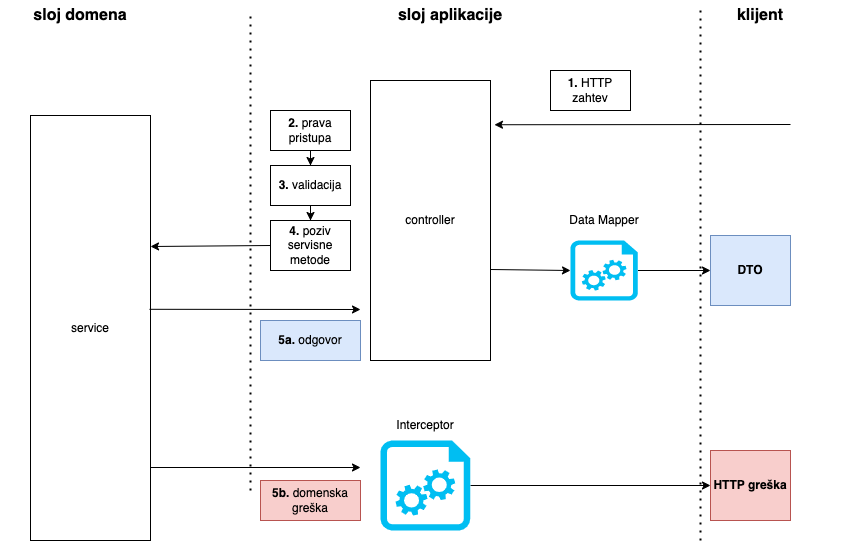
\includegraphics[width=1\textwidth]{docs/images/ch_2/applayer.png} 
  \caption{Aplikativni sloj}
  \label{fig:sample}
\end{figure}

što se tiče tehničkih aspekata, maksimalno je korišćeno metaprogramiranje za postizanje validacije i preslikavanja grešaka, kako bi se izbeglo repetitivno pisanje k\^{o}da. Presretači su suštinski manuelne provere tipa instance greške. Validacija je izvedena deklarativno kombinacijom biblioteka \textit{class-transformer} i \textit{class-validator}.

\begin{figure}[h]
\begin{lstlisting}[language=JavaScript, style=ES6, caption={presretač}]
return next.handle().pipe(
  catchError((error) => {
  if (error instanceof TicketNotFoundError) {
    throw new NotFoundException(error.getPayload());

    if (error instanceof NotAllowedToRemoveThisTagError) {
      throw new ForbiddenException(error.getPayload());
    }

    if (error instanceof DuplicateTagError) {
      throw new ConflictException(error.getPayload());
    }
\end{lstlisting}
\end{figure}




\begin{figure}[h]
\begin{lstlisting}[language=JavaScript, style=ES6, caption={validacija ulaznog DTO-a}]
export class AddTicketTagsDTO {
  @Validate(isValidObjectId, { each: true })
  @IsArray()
  tags: string[];
}
\end{lstlisting}
\end{figure}




    






% ------------------------------------------------------------------------------
\chapter{Frontend}
\section{Okruženje Next.js, serversko renderovanje React komponenti}
\section{Upravljanje stanjem aplikacije}
\section{Internacionalizacija}
\label{sec:intl}

% ------------------------------------------------------------------------------

% ------------------------------------------------------------------------------
\chapter{Analitika}
\section{Skladišta podataka, ETL procesi}
\section{Prikaz metrika, biblioteka Streamlit}
% ------------------------------------------------------------------------------

% ------------------------------------------------------------------------------
\chapter{Devops}
\section{Virtuelizacija, sistem Docker}
\section{nginx kao reverzni proksi}
% ------------------------------------------------------------------------------

% ------------------------------------------------------------------------------
\chapter{Zaključak}
% ------------------------------------------------------------------------------
% ------------------------------------------------------------------------------
% Literatura
% ------------------------------------------------------------------------------
\literatura

% ==============================================================================
% Završni deo teze i prilozi
\backmatter
% ==============================================================================

% ------------------------------------------------------------------------------
% Biografija kandidata
\begin{biografija}
/Lako ćemo to/
\end{biografija}
% ------------------------------------------------------------------------------

\end{document} 
